\chapter{Introduction to Algorithms}

\section{Basics of Algorithms}

\subsection{Definition of an Algorithm}
\begin{defi}[Algorithm Definition]
An algorithm is a finite sequence of well-defined instructions to solve a problem or perform a computation. Each step must be precise and executable in a finite amount of time.
\end{defi}

Algorithms are the foundation of programming and problem-solving in computer science. Their efficiency is often measured in terms of time complexity, which we introduce next.

\subsection{Theorem: Big-O Notation}
\begin{theorem}[Big-O Notation]
Let $f(n)$ and $g(n)$ be two non-negative functions. We say that $f(n)$ is $O(g(n))$ if there exist constants $c > 0$ and $n_0$ such that for all $n \geq n_0$, $f(n) \leq c \cdot g(n)$.
\end{theorem}

Big-O notation is used to classify algorithms according to their worst-case performance as the input size grows. For example, linear search has a time complexity of $O(n)$, meaning that the time it takes to complete grows linearly with the input size.

\subsection{Example: Time Complexity of Linear Search}
\begin{example}[Linear Search Time Complexity]
The time complexity of the linear search algorithm is $O(n)$. In the worst case, the algorithm checks each element in the array, resulting in a linear number of operations.
\end{example}

\subsection{Exercise: Analyze Linear Search}
\begin{exercise}
Implement the linear search algorithm in Python. Analyze its time complexity in both the best and worst cases.
\end{exercise}

\begin{example}[Time Complexity Chart]
    \centering
    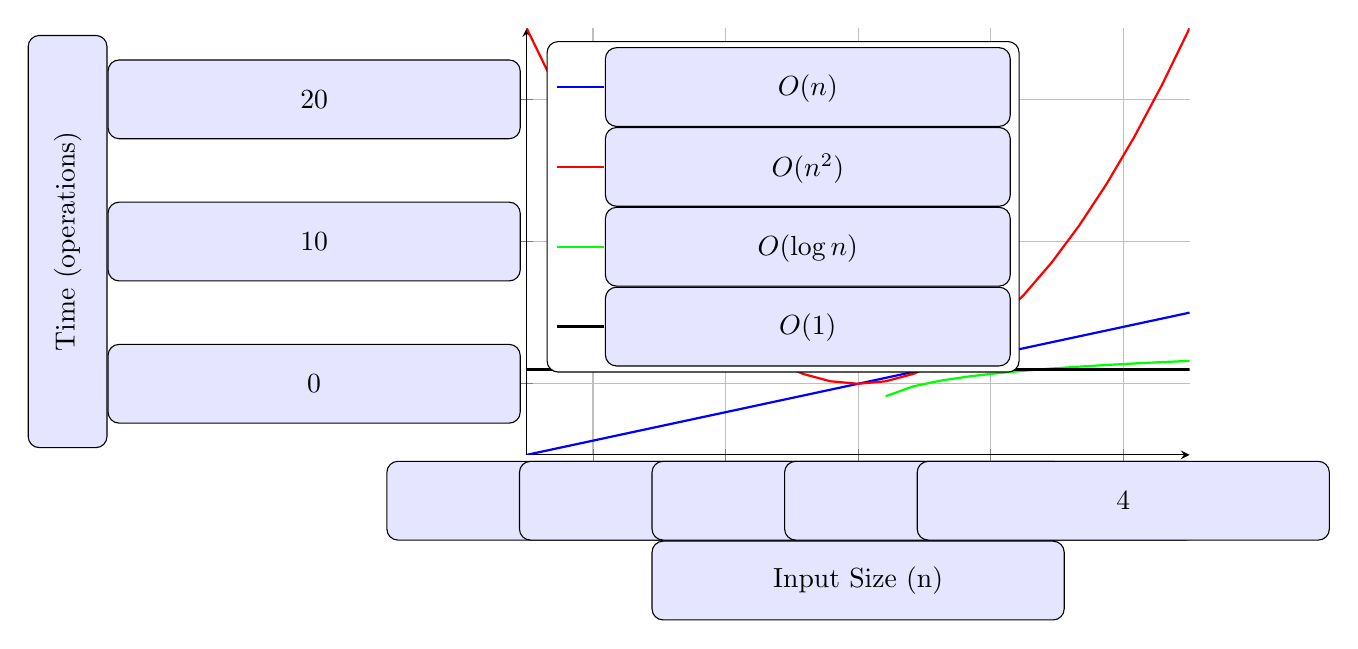
\begin{tikzpicture}
    \begin{axis}[
        xlabel={Input Size (n)},
        ylabel={Time (operations)},
        legend pos=north west,
        grid=major,
        axis lines=left,
        width=10cm,
        height=7cm
    ]
    % O(n)
    \addplot[blue, thick] {x};
    \addlegendentry{$O(n)$}

    % O(n^2)
    \addplot[red, thick] {x^2};
    \addlegendentry{$O(n^2)$}

    % O(log n)
    \addplot[green, thick] {ln(x)};
    \addlegendentry{$O(\log n)$}

    % O(1)
    \addplot[black, thick] {1};
    \addlegendentry{$O(1)$}
    \end{axis}
\end{tikzpicture}
  % Time Complexity Chart
\end{example}


\section{Sorting Algorithms}

\subsection{Theorem: Time Complexity of Sorting Algorithms}
\begin{theorem}[Time Complexity of Bubble Sort]
Bubble Sort is an $O(n^2)$ algorithm. In the worst case, Bubble Sort performs $n(n-1)/2$ comparisons.
\end{theorem}

\subsection{Proposition: Bubble Sort Efficiency}
\begin{prop}
In Bubble Sort, each pass through the array pushes the largest unsorted element to its correct position. This results in $O(n^2)$ time complexity, as every element may need to be compared multiple times.
\end{prop}

\subsection{Exercise: Implement Bubble Sort}
\begin{exercise}
Implement Bubble Sort in Python. Analyze its performance in both the best and worst cases.
\end{exercise}

\subsection{Python Code Snippet: Bubble Sort}
\begin{codesnippet}[Implementing Bubble Sort in Python]
\custominputminted{python}{Chapters/ch02/bubble_sort.py}
\end{codesnippet}


\begin{example}[Bubble Sort Steps]
    \centering
    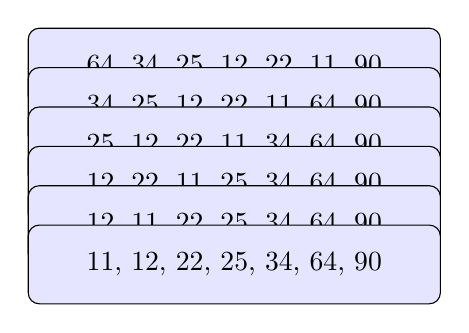
\begin{tikzpicture}
    % Initial array
    \node at (0, 1) {64, 34, 25, 12, 22, 11, 90};

    % After first pass
    \node at (0, 0.5) {34, 25, 12, 22, 11, 64, 90};

    % After second pass
    \node at (0, 0) {25, 12, 22, 11, 34, 64, 90};

    % After third pass
    \node at (0, -0.5) {12, 22, 11, 25, 34, 64, 90};

    % After fourth pass
    \node at (0, -1) {12, 11, 22, 25, 34, 64, 90};

    % Final sorted array
    \node at (0, -1.5) {11, 12, 22, 25, 34, 64, 90};
\end{tikzpicture}
  % Directly input the TikZ code
\end{example}


\section{Recursive Algorithms}

\subsection{Theorem: Recursion}
\begin{theorem}[Recursion Theorem]
A recursive algorithm solves a problem by breaking it down into smaller instances of the same problem, solving each instance recursively until reaching the base case.
\end{theorem}

\subsection{Example: Factorial Function}
\begin{example}[Factorial Function]
The factorial of a number $n$ is defined as:
\[
n! = \begin{cases}
1 & \text{if } n = 0, \\
n \cdot (n - 1)! & \text{if } n > 0.
\end{cases}
\]
\end{example}

\subsection{Exercise: Implement Recursive Factorial}
\begin{exercise}
Implement the factorial function in Python using recursion.
\end{exercise}

\subsection{Python Code Snippet: Recursive Factorial}
\begin{codesnippet}[Recursive Factorial in Python]
\custominputminted{python}{Chapters/ch02/recursive_factorial.py}
\end{codesnippet}

\begin{example}[Recursion Call Stack]
    \centering
    % 

\begin{tikzpicture}
    % Apply Helvetica font and style to all nodes
    \tikzstyle{every node}=[draw, fill=blue!10, rounded corners, minimum height=1cm, text width=5cm, align=center]

    % Define the matrix for the recursion stack
    \matrix (m) [matrix of nodes, column sep=0cm, row sep=0.3cm, nodes in empty cells]
    {
        \textbf{factorial(5)} \\
        \textbf{factorial(4)} \\
        \textbf{factorial(3)} \\
        \textbf{factorial(2)} \\
        \textbf{factorial(1)} \\
        \textbf{factorial(0)} \\
        \textbf{Return 1 (base case)} \\
    };

    % Draw arrows to indicate the recursion flow
    \draw[->, thick, blue] (m-1-1.south) -- (m-2-1.north);
    \draw[->, thick, blue] (m-2-1.south) -- (m-3-1.north);
    \draw[->, thick, blue] (m-3-1.south) -- (m-4-1.north);
    \draw[->, thick, blue] (m-4-1.south) -- (m-5-1.north);
    \draw[->, thick, blue] (m-5-1.south) -- (m-6-1.north);
    \draw[->, thick, blue] (m-6-1.south) -- (m-7-1.north);
\end{tikzpicture}
  % Recursive Call Stack
    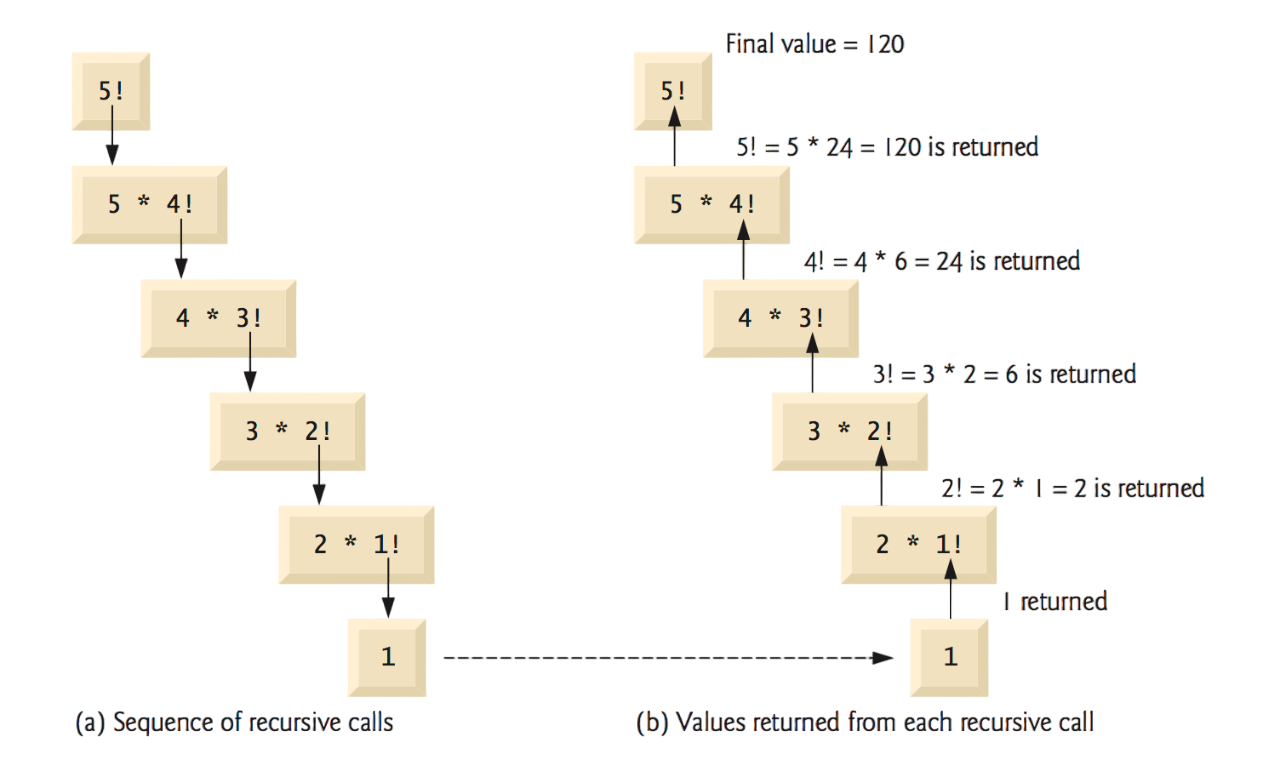
\includegraphics[width=0.7\textwidth]{Chapters/ch02/recursion_stack_image.png}  % Path to your image

\end{example}


\section{Dynamic Programming}

\subsection{Theorem: Principle of Optimality}
\begin{theorem}[Bellman's Principle of Optimality]
An optimal solution to a problem can be constructed from optimal solutions to its subproblems. This principle forms the basis of dynamic programming.
\end{theorem}

\subsection{Example: Fibonacci Sequence}
\begin{example}[Fibonacci Sequence Example]
The Fibonacci sequence is defined as:
\[
F(n) = \begin{cases}
0 & \text{if } n = 0, \\
1 & \text{if } n = 1, \\
F(n - 1) + F(n - 2) & \text{if } n \geq 2.
\end{cases}
\]
Using dynamic programming, we can compute $F(n)$ efficiently by storing previously computed values.
\end{example}

\subsection{Exercise: Implement Fibonacci Sequence}
\begin{exercise}
Implement the Fibonacci sequence in Python using both recursion and dynamic programming. Compare the performance of both implementations.
\end{exercise}

\subsection{Python Code Snippet: Fibonacci Sequence (Dynamic Programming)}
\begin{codesnippet}[Fibonacci Sequence in Python (DP)]
\custominputminted{python}{Chapters/ch02/fibonacci_dp.py}
\end{codesnippet}


\section{C++ Code Snippet: Sorting Algorithms}

\subsection{C++ Code Snippet: Quick Sort}
\begin{codesnippet}[Quick Sort in C++]
\custominputminted{cpp}{Chapters/ch02/quick_sort.cpp}
\end{codesnippet}


